\documentclass[10pt,conference,compsocconf]{IEEEtran}

\usepackage{hyperref}
\usepackage{graphicx}	% For figure environment

% Packages added by Joachim

%drow graph
\usepackage{fancybox}
\usepackage{tikz}
\usepackage{capt-of}
\usepackage{verbatim}

% cancel math expression
\usepackage{cancel}

% math
\usepackage{amsmath}

% url
\usepackage{hyperref}

%subfigure
\usepackage{subcaption}



\begin{document}
\title{PCML CS-433: Recommender System}

\author{
  Gael Lederrey, SCIPER \textcolor{red}{???}, gael.lederrey@epfl.ch \\
  Stefano Savar\`e, SCIPER \textcolor{red}{???}, stefano.savare@epfl.ch \\
  Joachim Muth, SCIPER 214757, joachim.muth@epfl.ch\\ \\
  \textit{School of Computer and Communication Sciences, EPF Lausanne, Switzerland}
}

\maketitle

%========================
\begin{abstract}

\end{abstract}

%========================
\section{Data description}

The data represent ratings from $10'000$ users on $1'000$ movies in an integer scale from 1 to 5. This scale represent the number of \textit{stars} given by the users, 1 being the lowest grade and 5 the best.

The training set used to train our algorithm contains $1'176'952$ ratings which represent around 12\% of possible filled ratings. 
An other $1'176'952$ ratings are hidden from us and must be predicted by our recommender algorithm.


%\begin{figure}[htbp]%------- PICTURE---------
%  \centering
%  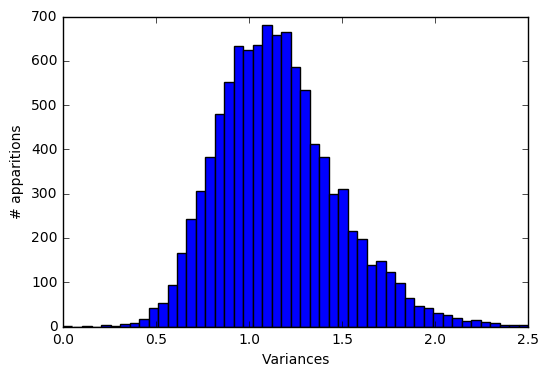
\includegraphics[width=0.9 \columnwidth]{img/Variances}
%  \caption{Distribution of variances of ratings per user.}
%  \vspace{-3mm}
%  \label{fig:denoise-fourier}
%\end{figure}
%\begin{figure}[htbp]
%  \centering
%  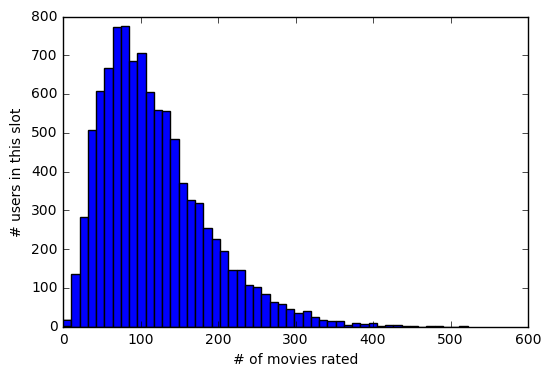
\includegraphics[width=0.9 \columnwidth]{img/Ratings}
%  \vspace{-3mm}
%  \caption{Number of movies rated per user.}
%  \label{fig:denoise-wavelet}
%\end{figure}


\begin{figure}[htbp]
    \centering
    \hspace{-0.6cm}
    \begin{subfigure}[t]{0.45\columnwidth}
        \centering
        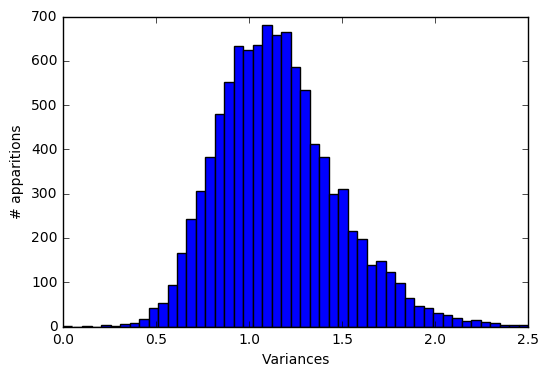
\includegraphics[height=1.2in]{img/Variances}
        \vspace{-3mm}
  \caption{Distribution of variances of ratings per user.}
    \end{subfigure}%
    \hspace{0.4cm}
    \begin{subfigure}[t]{0.45\columnwidth}
        \centering
        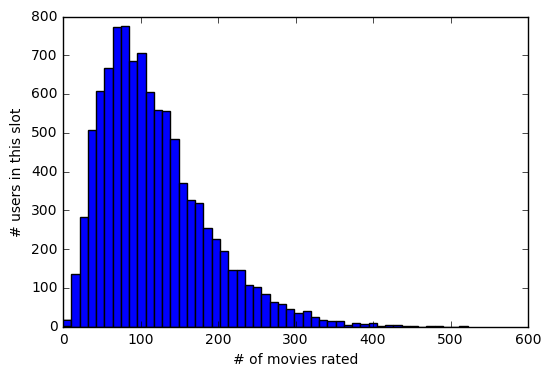
\includegraphics[height=1.2in]{img/Ratings}
        \vspace{-3mm}
        \caption{Number of movies rated per user.}
    \end{subfigure}
    \caption{Statistical description of data}
\end{figure}


%========================
\section{Data preprocessing}

\subsection{Search for spammers}

\subsection{Search for inactiv users}

\subsection{Normalization of user behaviour}
[To do: normalization of user mean and variance]



%========================
\section{Model selection}

\subsection{Models}
\subsubsection{Global mean}
\subsubsection{User/Movie mean}
\subsubsection{Matrix Factorization using Stochastic Gradient Descent}
\subsubsection{Alternativ Least Square}
\subsubsection{kNN item-based}
\subsubsection{Pareto Dominance and Collaborative Filtering Nearest Neighbors}

\subsection{Models benchmark}
[insert here a benchmark table for each method]

\subsection{Blending}


%========================
% \section{Discussion}



%========================
\section{Result}

\section{Discussion}


\bibliographystyle{IEEEtran}
\bibliography{literature}

\end{document}
